\documentclass[a4paper,12pt]{article}

\usepackage{estilos}

\pagestyle{empty}

\begin{document}

\begin{center}%
\begin{figure}[H]%
\begin{minipage}[H]{.55\columnwidth}%
\centering%
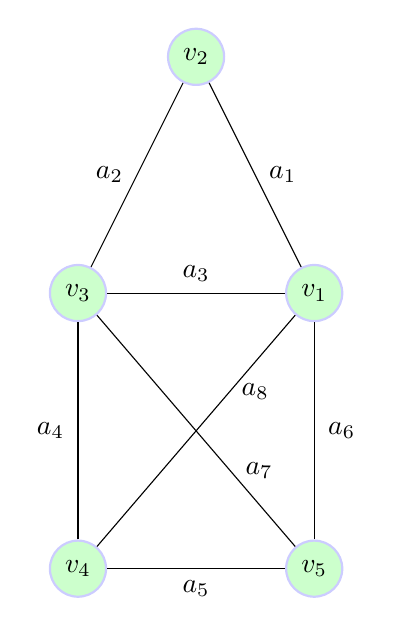
\begin{tikzpicture}{node distance=1.3cm,>=stealth',bend angle=45, auto}
  \tikzstyle{place}=[circle,thick,draw=blue!20,fill=green!20,minimum size=6mm]
  \tikzstyle{texto}=[]

  \begin{scope}

    \node [place] (c1) {$v_1$};

    \node [place] (c2) [above of=c1,xshift=-1.5cm,yshift=2cm] {$v_2$}
    edge [] node [xshift=.35cm] {$a_1$} (c1);

    \node [place] (c3) [left of=c1, xshift=-2cm] {$v_3$}
    edge [] node [yshift=.25cm] {$a_3$} (c1)
    edge [] node [xshift=-.35cm] {$a_2$} (c2);


    \node [place] (c4) [below of=c3,yshift=-2.5cm] {$v_4$}
    edge [] node [xshift=-.35cm] {$a_4$} (c3)
    edge [] node [yshift=.5cm,xshift=.75cm] {$a_8$} (c1);

    \node [place] (c5) [below of=c1,yshift=-2.5cm] {$v_5$}
    edge [] node [yshift=-.25cm] {$a_5$} (c4)
    edge [] node [xshift=.35cm] {$a_6$} (c1)
    edge [] node [yshift=-.5cm,xshift=.8cm] {$a_7$} (c3);
\end{scope}

\end{tikzpicture}
\end{minipage}%
\begin{minipage}{1cm}
\begin{center}
\[
 M =
 \begin{pmatrix}
  0 & 1 & 1 & 1 & 1 \\
  1 & 0 & 1 & 0 & 0 \\
  1 & 1 & 0 & 1 & 1 \\
  1 & 0 & 1 & 0 & 1 \\
  1 & 0 & 1 & 1 & 0
 \end{pmatrix}
\]
\end{center}
\end{minipage}
\end{figure}%
\end{center}%
\begin{figure}[H]
\begin{center}
\caption{Grafo con su representación en matriz de adyacencia}%
\end{center}
\end{figure}

 \end{document}
